%%%%%%%%%%%%%%%%%%%%%%%%%%%%%%%%%%%%%%%%%%%%%%%%%%%%%%%%%%%%%%%%%%%%%%%%
% Created 2020-09-30 Wed 15:22
% Intended LaTeX compiler: pdflatex
\documentclass[10pt,t]{beamer}
\usepackage[utf8]{inputenc}
\usepackage[T1]{fontenc}
\usepackage{graphicx}
\usepackage{grffile}
\usepackage{longtable}
\usepackage{wrapfig}
\usepackage{rotating}
\usepackage{amsmath}
\usepackage{textcomp}
\usepackage{amssymb}
\usepackage{capt-of}
\usepackage{hyperref}
\usetheme{default}
%\usepackage{scrextend}
%\usepackage{lipsum}

\author{S. Machado}
\date{\today}
\title{\large Twenty Years of Infrared Hyperspectral Satellite Measurements}
\subtitle{\footnotesize{From Spectroscopy to Climate}}
\date{\vspace{0.1in}\footnotesize{August 22-24,2022, Princeton NJ \vfill}}
\author{Sergio DeSouza-Machado\inst{1}}
\institute[UMBC]{\inst{1}UMBC JCET}
\input beamer_setup
\usetheme{metropolis}
\metroset{titleformat title=allcaps}
\renewcommand{\UrlFont}{\small\tt}
\renewcommand*{\UrlFont}{\footnotesize}
\tolerance=1000
\begin{document}

\maketitle

%%%%%%%%%%%%%%%%%%%%%%%%%%%%%%%%%%%%%%%%%%%%%%%%%%%%%%%%%%%%%%%%%%%%%%%%

\begin{frame}[shrink=2]{Outline}
%\begin{frame}{Outline}

\begin{block}{Thanks to :}
\vspace{0.25in}
Larrabee Strow (UMBC), Joao Teixeira (JPL) \newline
Chris Barnet (STM), Ryan Kramer (GSFC, UMBC) \newline
Scott Hannon, Howard Motteler, Chris Hepplewhite, Steve Buczkowski (UMBC) \newline
Marco Matricardi, Alan Geer (ECMWF), Guido Masiello (U. Basilicata, Italy)  \newline
Iouli Gordon (Harvard CFA), Eli Mlawer (AER), Manuel Lopez Puertas (U. of Granada, Spain)
\end{block}
\end{frame}

\begin{frame}[shrink=2]{Radiative Transfer codes : Accuracy vs Speed}
\begin{block}{Line by line codes : accuracy}
  \begin{itemize}
  \item Rich heritage
  \item GENLN2 (Dave Edwards) - 15 um CO2 line mixing from L.Strow
  \item LBLRTM (AER) water vapor continuum, N2/O2/other gases continuum, CO2/CH4 line mixing,spans MW to UV
  \item \textcolor{red}{kCARTA (UMBC)} \emph{latest HITRAN (2020), WV continuum + CO2/CH4 linemixing from LBLRTM, 
        focuses on IR, 25 seconds to do 605-2830 \wn at 0.0025 \wn resolution, 5 minutes to do 15-44000 \wn, jacobians, 
        fluxes, scattering}
  \item LBL codes typically use latest HITRAN/GEISA databases and are accurate, but too slow for operational use
  \end{itemize}
\end{block}

\begin{block}{Fast Models : speed}
  \begin{itemize}
  \item Parametrized fast codes for clear sky cloud clearing retrievals
  \item We use 49 regression profiles to span a variety of Earth climates; ECMWF has eg 25000
  \item \textcolor{red}{SARTA (UMBC)} \emph{used by NASA and NOAA for operational L2 retrievals of AIRS/CrIS, IASI}
  \item PCRTM (NASA Langley)
  \item RTTOVS (ECMWF) Data Assimilation
  \item Sigma IASI (U. of Basilicata, Italy) 
  \end{itemize}
\end{block}
\end{frame}

\begin{frame}[shrink=2]{Radiative Transfer Models (con'd)}
\begin{block}{Spectroscopy}
  \begin{itemize}
  \item HITRAN released every 4 years (into kCARTA within 6 months)
  \item Most recent update (2020) had largest changes to the O3 molecule line parameter from MW to UV, to yield
        consistent intensities (affects BT (10 um) by about 0.5 K)
  \item Uncertainty estimates from database yield $\delta(BT) \sim$ 0.2 K at TOA  
  \item Line mixing models and parameters for speed dependent Voigt line shapes, but we have not used them 
  \item AER will be releasing new WV continuum in Sept/Oct 2022 which will impact the window region; plus CO2/CH4 linemixing
        with H2020 database
  \item GEISA database (France) is very similar to HITRAN, also updates every couple years

  \end{itemize}
\end{block}

\begin{block}{Non local thermodynamic equilibrium}
  \begin{itemize}
  \item NLTE mostly affects the 4.3 um CO2 band (nadir sounding)
  \item Manuel Lopez Puertas (Granada, Spain) has developed models upper atmosphere NLTE vibrational temperatures
  \item UMBC developed a fast model using this database
  \item We don't worry too much about strat/meso temperatures and atmospheric concentrations (cannot see with nadir sounders)
  \end{itemize}
\end{block}
\end{frame}

%%%%%%%%%%%%%%%%%%%%%%%%%%%%%%%%%%%%%%%%%%%%%%%%%%%%%%%%%%%%%%%%%%%%%%%%
\begin{frame}{Impact of Spectral Uncertainties}

\begin{block}{}
$\Delta$ (BT) for perturbations to (a) wavenumber and (b)
  line shift due to pressure parameters. The top and bottom panels show mean and
  standard deviations of the changes, while the black curves are the
  AIRS NeDT at 250 K. Most of the perturbations were below the 0.1 \wn level.
\begin{figure}
\begin{center}
\includegraphics[width=0.475\textwidth]{../../SUBMITPAPERS/PAPER1_KCARTA/UNC/strengthplus_airsV2.pdf}
\includegraphics[width=0.475\textwidth]{../../SUBMITPAPERS/PAPER1_KCARTA/UNC/broadplus_airsV2.pdf}
\end{center}
\end{figure}
\end{block}
\end{frame}

\begin{frame}{Comparing Spectral Databases}

\begin{block}{}
 Left panel (a) : H2016 versus GEISA 2015 (blue) and H2012
  (red). The black curve is the AIRS NeDT. Right panel (b) : 15 \um CO2
  line mixing differences, compared to LBLRTM 12.4 (red) and UMBCLBL
  (blue). For both sets of plots the top is the mean differences
  versus the control (HITRAN 2016 with \cd,\methane line mixing from LBLRTM v12.8
\begin{figure}
\begin{center}
\includegraphics[width=0.45\textwidth]{../../SUBMITPAPERS/PAPER1_KCARTA/GEISA_HTRAN/hitran_geisaV2.pdf}
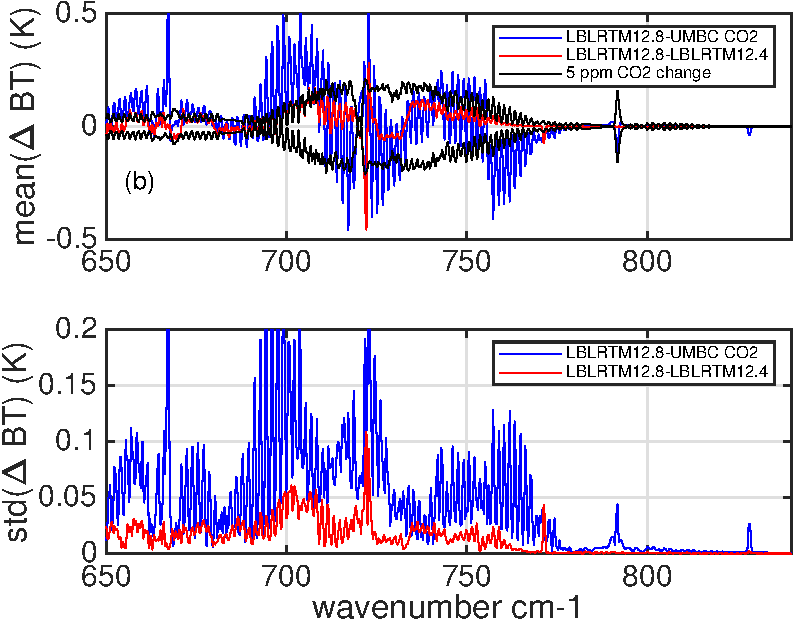
\includegraphics[width=0.45\textwidth]{../../SUBMITPAPERS/PAPER1_KCARTA/GEISA_HTRAN/co2_linemix_flavorsV2.pdf}
\end{center}
\end{figure}
\end{block}
\end{frame}

%%%%%%%%%%%%%%%%%%%%%%%%%%%%%%%%%%%%%%%%%%%%%%%%%%%%%%%%%%%%%%%%%%%%%%%%

\begin{frame}[shrink=2]{Radiative Transfer Models (con'd)}
\begin{block}{Surface properties}
  \begin{itemize}
  \item Ocean emissivity : Masuda model (1988, updated in 2006) as a function of wind speed
  \item Land Emissivity : Dan Zhou (NASA Langley) and CAMEL (U. Wisc) as a function of month/year
  \item Sea surface reflectivity : Nick Nalli is working on developing sun glint models, but these would mostly affect the SWIR
  \end{itemize}
\end{block}

\begin{block}{Scattering}
  \begin{itemize}
  \item DISORT (Stamnes et. al. 1988) : Very accurate, but slow
  \item Parameterization for LongWave Scattering (Chou et. al 1999) : Very fast, about 2 K errors across IR spectrum for DCC
  \item Successive Orders of Scattering : mostly used for NIR/Vis (to my knowledge)
  \item Adjustment to Chou (Tang. et. al 2018) : Very fast, working on a better parameterization
  \end{itemize}
\end{block}

\begin{block}{Clouds and Aerosols}
  \begin{itemize}
  \item Complex cloud models (Maximum Random Overlap) give smooth heating profiles, multiple sub pixels are computationally costly
  \item Simple cloud models (TwoSlab) are fast and quite accurate, but can give spikes at cloud slab boundaries
  \item RRTM (AER) has in-built fast RTA for flux calculations, handles scattering, 3-4 gaussian angles
  \item ecRad (Robin Hogan, ECMWF) developed flux model for ECWMF
  \item Typically only dust (4 um large aerosols) affects IR radiances in the window region, though IASI has seen 
        effects of eg sulphates and smoke in the window region
  \end{itemize}
\end{block}
\end{frame}

\begin{frame}[shrink=2]{Operational Retrievals}
\begin{block}{Typical Hyperspectral Sounder}
  \begin{itemize}
  \item Atmospheric Infrared Sounder, almost continually operational since September 2002
  \item Diffraction grating instrument, 2378 channels, 500 pristine channels 
        (Strow/Machado AMT 2018) of resolution about 0.5-2 cm-1, 15 km diameter footprint at nadir
  \item 1.30 am/pm equator crossing time, twice daily views of Earth, 16 day repeat cycle
  \item Takes 90 cross track x 135 along track spectral every 6 minutes
  \item Roughly 2.92 million spectra daily x 20 years!
  \end{itemize}
\end{block}

\begin{block}{Typical Operational Retrieval}
  \begin{itemize}
    \item Quite difficult to process this! 
    \item Plus there is cloud contamination
    \item Cloud clearing process ``removes'' effects of clouds
       \begin{itemize}
          \item reduces spatial resolution from 15 km to 3x3 or 45 km
          \item ``increases'' spectral noise, and hence retrieval uncertainty
          \item fails when all scenes are uniform eg clear scene or uniform dust
          \item uses black clouds (ie not spectrally realistic)
       \end{itemize}
    \item Typical AIRS v7 retrievals (T(z), WV(z), surface temp, trace gases, clouds, surface emissivity) takes about 2 seconds
    \item Complicated QA, and first guess from neural network
    \item NOAA CLIMCAPS first guess uses documented MERRA2 as first guess, simpler QA, about 0.7 seconds/FOR
    \item Alternatives
    \begin{itemize}
      \item EUMETSAT does hole hunting to look for clear scenes
      \item Regression based allsky retrievals (Bill Smith UWisc/Hampton U)
      \item Single footprint allsky retrievals (JPL Irion, Langley Liu, UMBC)
      \item Artificial Intelligence allsky retrievals (NOAA Maddy/Boukabara)
    \end{itemize}
  \end{itemize}
\end{block}
\end{frame}
  
\end{document}

%%%%%%%%%%%%%%%%%%%%%%%%%%%%%%%%%%%%%%%%%%%%%%%%%%%%%%%%%%%%%%%%%%%%%%%% THE END %%%%%%%%%%%%%%%%%%%%%%%%%

%%%%%%%%%%%%%%%%%%%%%%%%%%%%%%%%%%%%%%%%%%%%%%%%%%%%%%%%%%%%%%%%%%%%%%%%
\begin{block}{Approach:}
\begin{itemize}
\item Long-term: Retrieval geophysical anomalies \emph{directly} from radiance anomalies to enhance climate accuracy
\item This talk:
\begin{itemize}
\item By-pass anomaly retrievals (time-series) and focus on 19-year linear trend retrievals directly from radiance linear trends.
\end{itemize}
\item Trends presented here will serve as closure tests for future anomaly trend retrievals
\end{itemize}
\end{block}

\begin{block}{Feedbacks:}
\begin{itemize}
\item Use retrieved linear trends to estimate climate feedbacks
\end{itemize}
\end{block}

\end{frame}

%%%%%%%%%%%%%%%%%%%%%%%%%%%%%%%%%%%%%%%%%%%%%%%%%%%%%%%%%%%%%%%%%%%%%%%%

\begin{frame}{OEM Retrievals}
\begin{block}{}
\begin{itemize}

\item {\large Use trends from hottest (clearest) obs and/or the
      mean (allsky) observations}
\item Use 20 layers and zero \emph{a-priori}
\item fix trace gases (CO2, N2O, CH4) to ESRL rates; retrieve T(z),WV(z),O3(z),surf temp trends
\item Compare against following datasets, starting Sept 2002
  \begin{itemize}
  \item ERA5 monthly (ERA-I daily stopped August 2019)
  \item AIRS3 L3 monthly
  \item CMIP6 : historical runs all forcings, monthly to Aug 2014
  \end{itemize}
\item Timings on UMBC HPC cluster
  \begin{itemize}
    \item All the hard work in tiling 18 years of AIRS data done, now all we do is add on a month or so at a time
    \item Run off trends/anomalies (day or so)
    \item 64 $\times$ 72 trend retrievals $\rightarrow$ 15 mins, 64 zonal averages $\rightarrow$ 1 min
    \item compare to re-processing AIRS L2 or L3 ....
  \end{itemize}
\end{itemize}
\end{block}
\end{frame}

%%%%%%%%%%%%%%%%%%%%%%%%%%%%%%%%%%%%%%%%%%%%%%%%%%%%%%%%%%%%%%%%%%%%%%%%
\begin{frame}{OLR in the Far-IR}
\begin{block}{}

\vspace{-0.1in}
\begin{columns}

\begin{column}{0.55\columnwidth}
\begin{block}{}
\vspace{-0.1in}
\begin{center}
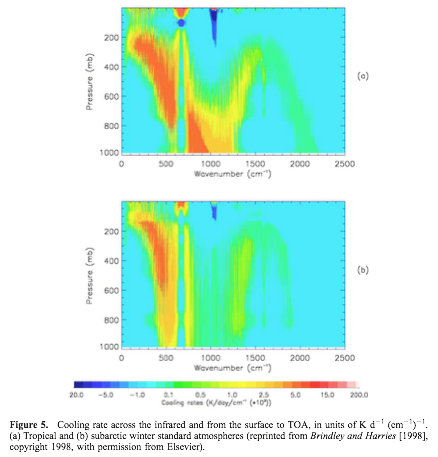
\includegraphics[width=\linewidth]{image_spectralOLR.png}
\end{center}
\end{block}
\end{column}

\begin{column}{0.55\columnwidth}
\begin{block}{}
\begin{itemize}
\item Far-IR WV emission dominates atmospheric cooling, esp. in descending tropical regions
\item AIRS observed mid-IR WV has sensitivity where (WV) OLR is large in far-IR
\item Allows computation of feedbacks from AIRS retrievals using computed OLR driven by mid-IR WV retrievals
\end{itemize}
\end{block}
\end{column}

\end{columns}

\end{block}
\end{frame}

%%%%%%%%%%%%%%%%%%%%%%%%%%%%%%%%%%%%%%%%%%%%%%%%%%%%%%%%%%%%%%%%%%%%%%%%

\begin{frame}{Night ALL Spectral Rates}

% \textcolor{red}{Green curve is very similar to MEAN AIRS obs trends shown by Larrabee in previous talk!}

\begin{center}
\includegraphics[width=0.95\linewidth]{Figs_STMOct2021/spectral_all_N_ratesV2.png}
\end{center}
\end{frame}


\begin{frame}{Simulated tropical $dBT(\nu)/dt$}

\vspace{-0.1in}
\begin{columns}

\begin{column}{0.75\columnwidth}
\begin{block}{}
\vspace{-0.1in}
\begin{center}
\includegraphics[width=0.975\linewidth]{Figs_STMOct2021/delta_BT_with_WVv3.pdf}
\end{center}
\end{block}
\end{column}

\begin{column}{0.35\columnwidth}
\begin{block}{}

\begin{itemize}
\item Realistic dT(z)/dt, dCO2/dt = 2.2 ppm/yr
\item WVfrac changes to (a) keep RH constant, or \newline (b) reduce RH
\end{itemize}
\end{block}
\end{column}

\end{columns}

\end{frame}

%%%%%%%%%%%%%%%%%%%%%%%%%%%%%%%%%%%%%%%%%%%%%%%%%%%%%%%%%%%%%%%%%%%%%%%%

\begin{frame}{Is $\delta$ RH = 0}


{\bf Climate Change 2007: Working Group I: The Physical Science Basis} \newline
https://archive.ipcc.ch/publications\_and\_data/ar4/wg1/en/ch8s8-6-3-1.html \newline

Understanding processes determining the distribution and variability
in RH is therefore central to understanding of the water vapour-lapse
rate feedback. \emph{To a first approximation, GCM simulations indeed
maintain a roughly unchanged distribution of RH under greenhouse gas
forcing. More precisely, a small but widespread RH decrease in GCM
simulations typically reduces feedback strength slightly compared with
a constant RH response} (Colman, 2004; Soden and Held, 2006; Figure
8.14).

\end{frame}
%%%%%%%%%%%%%%%%%%%%%%%%%%%%%%%%%%%%%%%%%%%%%%%%%%%%%%%%%%%%%%%%%%%%%%%%

\begin{frame}{Surface Temperature Trends K/yr}
\begin{footnotesize}
\begin{itemize}
\item May 2021 STM excellent agreement with GISTEMP, HADCRU4
\item They do not see AIRS L3 cooling in the Antartic
\item allsky trends $\sim$ hottest trends on average, much more spatial variation
\end{itemize}
\end{footnotesize}
\begin{center}
\includegraphics[width=0.925\linewidth]{Figs_STMOct2021/skt_rates_tiled.png}
\end{center}
\end{frame}

\begin{frame}{Night Land Atmospheric temperature Trends K/yr}
\begin{center}
\includegraphics[width=0.95\linewidth]{Figs_STMOct2021/tiled_land_N_T_trend.png}
\end{center}
\end{frame}

\begin{frame}{Night Ocean Atmospheric temperature Trends K/yr}
\begin{center}
\includegraphics[width=0.95\linewidth]{Figs_STMOct2021/tiled_ocean_N_T_trend.png}
\end{center}
\end{frame}

%\begin{frame}{Night All} : dT/dt}
%\begin{center}
%\includegraphics[width=0.95\linewidth]{Figs_STMOct2021/tiled_all_N_T_trend.png}
%\end{center}
%\end{frame}



\begin{frame}{Night Land dWVfrac/dt 1/yr}
\begin{center}
\includegraphics[width=0.95\linewidth]{Figs_STMOct2021/tiled_land_N_WVfrac_trend.png}
\end{center}
\end{frame}

\begin{frame}{Night Ocean dWVfrac/dt 1/yr}
\begin{center}
\includegraphics[width=0.95\linewidth]{Figs_STMOct2021/tiled_ocean_N_WVfrac_trend.png}
\end{center}
\end{frame}

%\begin{frame}{Night All} : dWVfrac/dt}
%\begin{center}
%\includegraphics[width=0.95\linewidth]{Figs_STMOct2021/tiled_all_N_WVfrac_trend.png}
%\end{center}
%\end{frame}

\begin{frame}{Night Land : dRH/dt percent/yr}
\begin{center}
\includegraphics[width=0.95\linewidth]{Figs_STMOct2021/tiled_land_N_RH_trend.png}
\end{center}
\end{frame}

\begin{frame}{Night Ocean : dRH/dt percent/year}
\begin{center}
\includegraphics[width=0.95\linewidth]{Figs_STMOct2021/tiled_ocean_N_RH_trend.png}
\end{center}
\end{frame}

%\begin{frame}{Night All} : dRH/dt}
%\begin{center}
%\includegraphics[width=0.95\linewidth]{Figs_STMOct2021/tiled_all_N_RH_trend.png}
%\end{center}
%\end{frame}

\begin{frame}{Night Land}
\begin{center}
\includegraphics[width=0.95\linewidth,height=0.875\textheight]{Figs_STMOct2021//tiled_land_N_T_RH_WVfracrates.png}
\end{center}
\end{frame}

\begin{frame}{Night Ocean}
\begin{center}
\includegraphics[width=0.95\linewidth,height=0.875\textheight]{Figs_STMOct2021//tiled_ocean_N_T_RH_WVfracrates.png}
\end{center}
\end{frame}

%\begin{frame}{Night All}}
%\label{all:trends}
%\begin{center}
%\includegraphics[width=0.95\linewidth,height=0.875\textheight]{Figs_STMOct2021//tiled_all_N_T_RH_WVfracrates.png}
%\end{center}
%\end{frame}

%%%%%%%%%%%%%%%%%%%%%%%%%%%%%%%%%%%%%%%%%%%%%%%%%%%%%%%%%%%%%%%%%%%%%%%%
\begin{frame}{Night All : Spectral closure with unc}
\begin{footnotesize}
Obs uncertainty : fitting the 16 day avg data, has all inter-anual variability \newline
Retrieval+Model uncertainty : unc in geophysical trends $\rightarrow$ spectra \newline
\end{footnotesize}
\begin{center}
%\includegraphics[width=0.95\linewidth,height=0.625\textheight]{~/MATLABCODE/oem_pkg_run/AIRS_gridded_STM_May2021_trendsonlyCLR_zonalavg/spectral_plot_with_unc2.pdf}
\includegraphics[width=0.95\linewidth,height=0.625\textheight]{~/MATLABCODE/oem_pkg_run/AIRS_gridded_STM_May2021_trendsonlyCLR/spectral_plot_with_unc2_64x72.pdf}
\end{center}
\end{frame}
%%%%%%%%%%%%%%%%%%%%%%%%%%%%%%%%%%%%%%%%%%%%%%%%%%%%%%%%%%%%%%%%%%%%%%%%

\begin{frame}{Feedback Parameters}

{\small 
Use one sided OLR clear sky changes from ecRad (R. Hogan, ECMWF) and equations from 
Jevanjee, Koll, Lutsko, ``Simpson's Law and the Spectral Cancellation of Climate Feedbacks'', GRL 2020}

\vspace{-0.25in}
\begin{columns}

\begin{column}{0.55\columnwidth}
\begin{block}{}
\vspace{-0.1in}
\begin{center}
\includegraphics[width=0.975\linewidth]{Figs_STMOct2021//tiled_feedbackparams.pdf}
\end{center}
\end{block}
\end{column}

\begin{column}{0.55\columnwidth}
\begin{block}{}
\begin{itemize}
\item $\lambda = -\frac{d(OLR(xf)-OLR(x0))}{d(ST)}$
\item Preliminary work
%\item Used same underlying X0 geophysical (unperturbed state)
%\item Perturb using dST/dt,dT(z)/dt,dWVfrac/dt $\rightarrow \lambda$
\item Planck : IPCC $\sim$ -3.3 W/m2/K
\item SKT : use window region Planck!
\item WV and Lapse feedback : UMBC and AIRS L3 are obs, quite similar!
\end{itemize}
\end{block}
\end{column}

\end{columns}
\end{frame}

\begin{frame}{Feedback Values (W/m2/K)}

Notable differences between \emph{Observations} versus Models

\begin{center}
\begin{tabular}{ c c c c c}
\hline
        &   Planck   &     Lapse    &      WV    &        SKT  \\
\hline
\emph{UMBC}    & -3.89  &   \emph{0.93}   &   \emph{0.27} &   -1.18 \\
\emph{AIRS v7} & -3.89  &   \emph{1.26}   &   \emph{0.46} &   -1.18 \\
ERA5    & -3.89  &   0.13   &   1.13 &   -1.18 \\
CMIP6   & -3.89  &  -0.21   &   1.95 &   -1.18 \\
\hline
\hline
\emph{AIRS v6} & & \emph{0.77} & \emph{1.05} & \\
\emph{AIRS v7} & & \emph{0.67} & \emph{0.73} & \\
MERRA2  & & -0.03 & 1.61 & \\
ERA5    & & -0.46 & 1.83 & \\
\hline
\end{tabular}
\end{center}
Haozhe He, 12 pm talk \emph{Evaluating Observational Constraints on Intermodel Spread in
Cloud, Temperature and Humidity Feedbacks}

\end{frame}

%%%%%%%%%%%%%%%%%%%%%%%%%%%%%%%%%%%%%%%%%%%%%%%%%%%%%%%%%%%%%%%%%%%%%%%%

\begin{frame}{Conclusions}

\begin{block}{Conclusions}
\begin{itemize}

\item \textcolor{red}{Zero \emph{a-priori}} for thermodynamic trends (19 years of AIRS data)

\item \textcolor{red}{Spectral closure indicative that UMBC retrievals are correct}
\begin{itemize}
\item same results using trends from clearest obs (4608 tiles), clearest obs (64 zonal averages), mean obs (4608 tiles)
\item used results for deriving feedbacks parameters
\end{itemize}

\item ST (not shown) and T(z,lat) trends 
%\begin{localsize}{8}
\begin{itemize}
\item are approximately same for UMBC, AIRS L3, ERA5; CMIP6 shows more warming in N. Polar
\item more warming over ocean than land
\end{itemize}
%\end{localsize}

\item WVfrac(z,lat) and RH(z,lat) trends 
%\begin{localsize}{8}
\begin{itemize}
\item UMBC shows tiniest increases, not large enough to offset T increase, so RH decreases overall
\item So does AIRS L3!
\item ERA5 and CMIP6 seem to imply that RH is $\sim$ constant
\end{itemize}
%\end{localsize}

\item Feedback parameters from obs different from models
\end{itemize}
\end{block}

\end{frame}
\end{document}
%%%%%%%%%%%%%%%%%%%%%%%%%%%%%%%%%%%%%%%%%%%%%%%%%%%%%%%%%%%%%%%%%%%%%%%%
